\documentclass[14pt]{report}

\usepackage{geometry}
\usepackage[utf8]{inputenc}
\usepackage{amsmath}
\usepackage{amsfonts}
\usepackage{amssymb}
\usepackage{graphicx}
\usepackage[utf8]{inputenc}
\usepackage{amsmath}
\usepackage{amsfonts}
\usepackage{amssymb}
\usepackage[shortlabels]{enumitem}
\usepackage{listings}
\usepackage{xcolor}
\usepackage[most]{tcolorbox}
\usepackage{mathtools}
\usepackage{float}
\usepackage[colorlinks=false, linktocpage=true]{hyperref}
\usepackage{enumitem}

\usepackage{booktabs}% http://ctan.org/pkg/booktabs
\newcommand{\tabitem}{~~\llap{\textbullet}~~}
\usepackage{longtable}
 
\usepackage{caption}
\DeclareCaptionType{code}[Code Listing][List of Code Listings] 

\definecolor{codegreen}{rgb}{0,0.6,0}
\definecolor{codegray}{rgb}{0.5,0.5,0.5}
\definecolor{codepurple}{rgb}{0.58,0,0.82}
\definecolor{backcolour}{rgb}{0.95,0.95,0.92}
 
\lstdefinestyle{mystyle}{
    backgroundcolor=\color{backcolour},   
    commentstyle=\color{codegreen},
    keywordstyle=\color{magenta},
    numberstyle=\tiny\color{codegray},
    stringstyle=\color{codepurple},
    basicstyle=\ttfamily\footnotesize,
    breakatwhitespace=false,         
    breaklines=true,                 
    captionpos=b,                    
    keepspaces=true,                 
    numbers=left,                    
    numbersep=5pt,                  
    showspaces=false,                
    showstringspaces=false,
    showtabs=false,                  
    tabsize=2
}
 
\lstset{style=mystyle}

\setlength{\parindent}{0em}
\setlength{\parskip}{1em}

\author{Brian Rashap, Ph.D.}
\title{PHYS 1320 - Calculus-based Physics II}

\geometry{letterpaper, portrait, margin=0.75in}

\begin{document}

\begin{center}
\textbf{Physics 1320 - Calculus-based Physics II \\ Summer 2022 \\ Midterm Exam II}
\end{center}

\textbf{Question 1} (15 pts)

Consider a segment of AWG 12 (diameter = 2.052mm) copper wire in a circuit that is $20m$ long. The potential difference from one end to the end of the wire is $12V$.

\begin{figure}[H]
\begin{center}
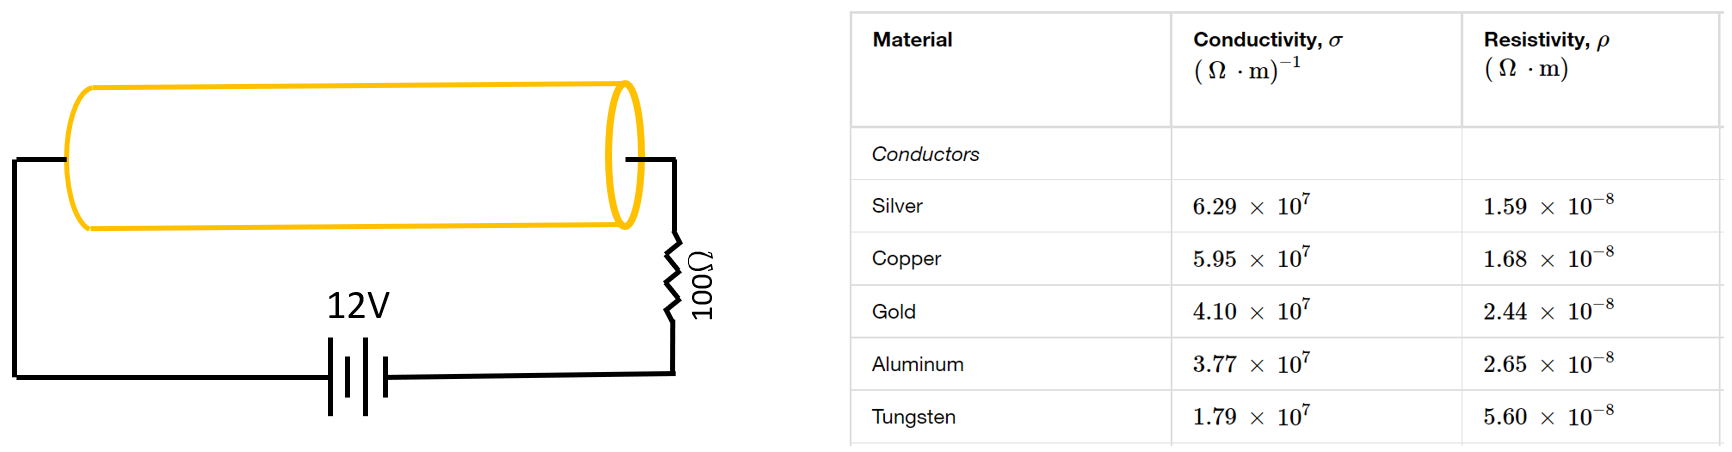
\includegraphics[scale=0.55]{exam2_1.png}
\end{center}
\end{figure}

\begin{enumerate}[label=\Alph*]
\item What is the resistance of this segment of wire?
\item For an aluminum wire of the same length, what diameter is required to match the resistance of the copper wire?
\item How much energy is used by this segment of wire?
\item Where does this energy go?
\end{enumerate}

\textbf{Question 2} (15 pts)

Consider the below circuit:

\begin{figure}[H]
\begin{center}
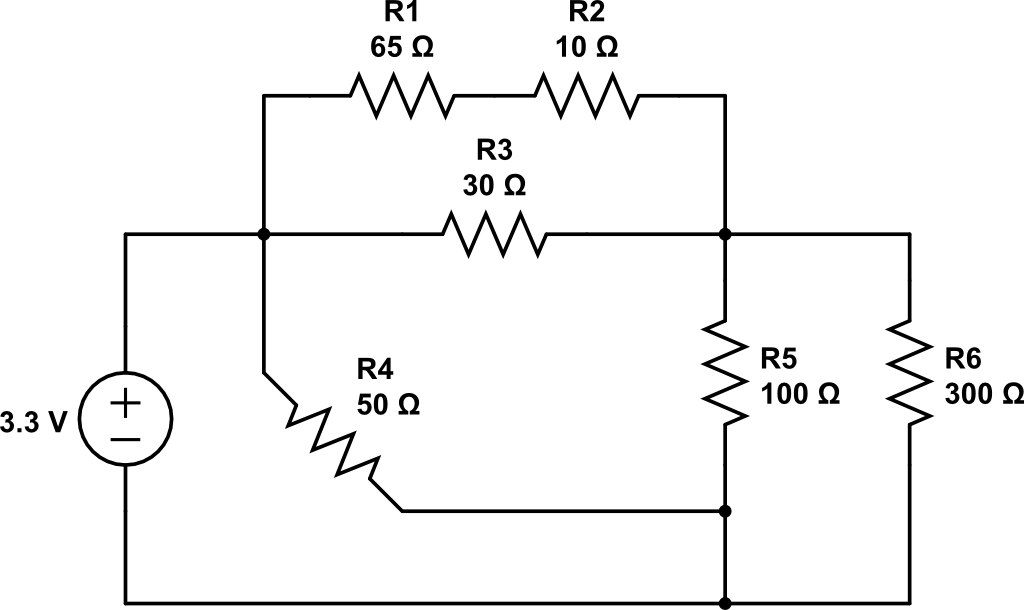
\includegraphics[scale=0.40]{circuit_2_2.png}
\end{center}
\end{figure}

\begin{enumerate}[label=\Alph*]
\item What is the total current flowing from the power supply?
\item What is the voltage across resistor $R_2$?
\item What is the current through resistor $R_6$?
\end{enumerate}

\newpage
\textbf{Question 3} (20 pts)

Consider the circuit below with a power supply $V=12V$, $R_1 = 10k \Omega$, $R_2 = 3.3k \Omega$, $C_1 = 180 \mu F$, and $C_2 = 120 \mu F$. 

\begin{figure}[H]
\begin{center}
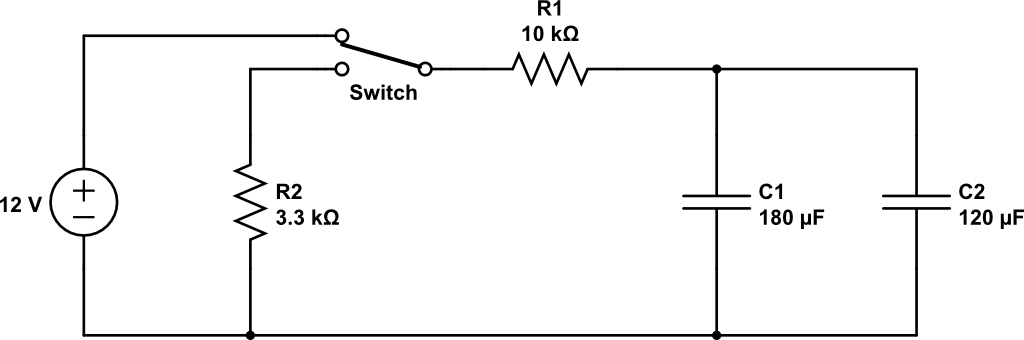
\includegraphics[scale=0.65]{exam2_3.png}
\end{center}
\end{figure}

Assume that the switch starts open (connected neither to the power supply nor the resistor $R_2$). It closes to the power supply at time = 5 seconds. And, then at time = 14 seconds it switch over to connect to the resistor $R_2$. 

\begin{enumerate}[label=\Alph*]
\item What is the charge on capacitor $C_2$ at time = 11 seconds?
\item What is the voltage across capacitor $C_1$ at time = 20 seconds?
\end{enumerate}

\textbf{Question 4} (15 pts)

Consider a magnetic field of magnitude $2.73 T$ that is parallel to the positive z-axis. For each of the following situations, calculate the force vector acting upon the particle.

\begin{enumerate}[label=\Alph*]
\item An electron moving in the negative y direction with a velocity of $4.2 \frac{m}{s}.$
\item A proton moving in the negative z direction with a velocity of $8.99 \frac{m}{s}.$
\item An alpha-particle (two protons and two electrons) moving with a velocity of $(-3 \hat{i} + 4 \hat{j} - 5 \hat{k}) \frac{m}{s}$
\end{enumerate}

\textit{Note: the mass of a proton is $m_p = 1.637 \cdot 10^{-27} kg$ and the mass of a electron is $9.11 \cdot 10^{-31} kg$. The charge on an electron is $1.602 \cdot 10^{-19} C$.}

\newpage
\textbf{Question 5} (15 pts)

Consider a right triangle with sides of $3cm$ and $4cm$ carrying $5A$ of current as shown in the figure below. It is placed in a $80mT$ magnetic field at an angle of $45^o$.

\begin{figure}[H]
\begin{center}
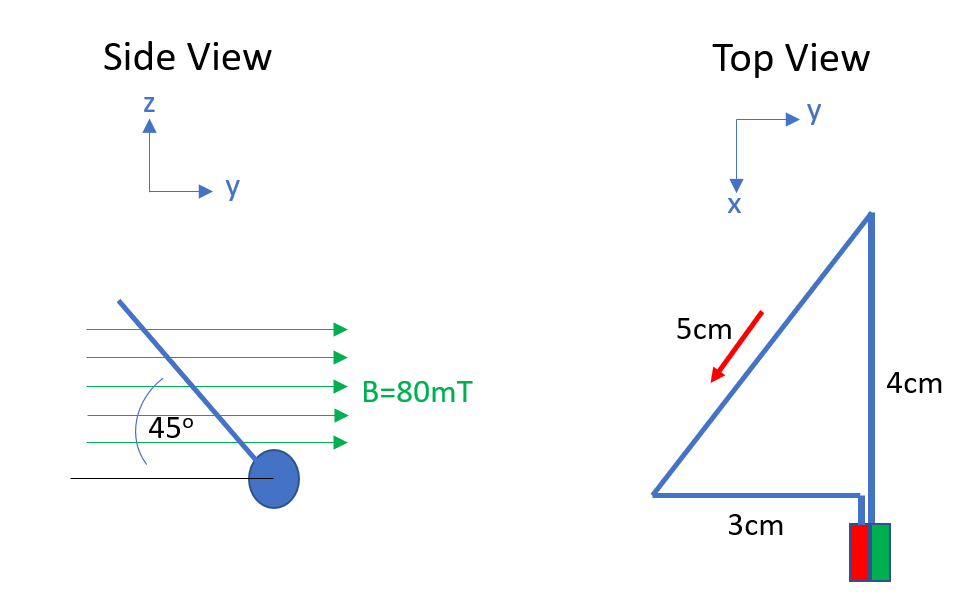
\includegraphics[scale=0.80]{magneticdipole.png}
\end{center}
\end{figure}

\begin{enumerate}[label=\Alph*]
\item What is the force on each of the three sides of the triangle?
\item What is the magnetic dipole moment of this current-carrying loop?
\item What is the torque on this current-carrying loop?
\end{enumerate}



\textbf{Question 6} (20 pts)

Consider the below mass spectrometer with the following fields with $E = 12,500 \frac{V}{m}$, $B = 0.01T$, and $B_0 = 1.404 T$ in the directions shown in the Figure below. 

\begin{figure}[H]
\begin{center}
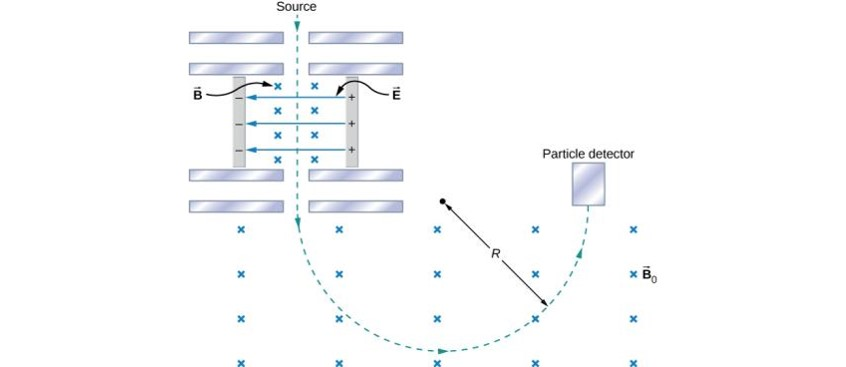
\includegraphics[scale=0.60]{fig_11_19.jpg}
\end{center}
\end{figure}

\begin{enumerate} [label=\Alph*]
\item Describe qualitatively how the velocity selector portion of the mass spectrometer works.
\item What is the velocity of a particle emerging from the velocity selector?
\item A gas chromatography system breaks the source gas into constituent atoms and ionizes them. These ions then enter the mass spectrometer. An equal number of ions (singularly charged) hit a detector at radius $12.91cm$ and $14.75cm$, what is the mass of each type of ion?
\item Given the table at the end of this exam, what is the original gas that was fed into the gas chromatogrphy system? (Note: $1$ AMU $= 1.66 * 10^{-27} kg$).

\end{enumerate}

\textbf{Question 7 - Extra Credit} (5pts)
\begin{enumerate}[label=\Alph*]
\item How much horsepower can a horse exert over a short period of time?
\item If the horse exerts its maximum pull for 5 minutes, how much Energy does it use. (Note: one horsepower equals 745.7 W).
\end{enumerate}

\textbf{Reference: Atomic Mass Table}

\begin{figure}[H]
\begin{center}
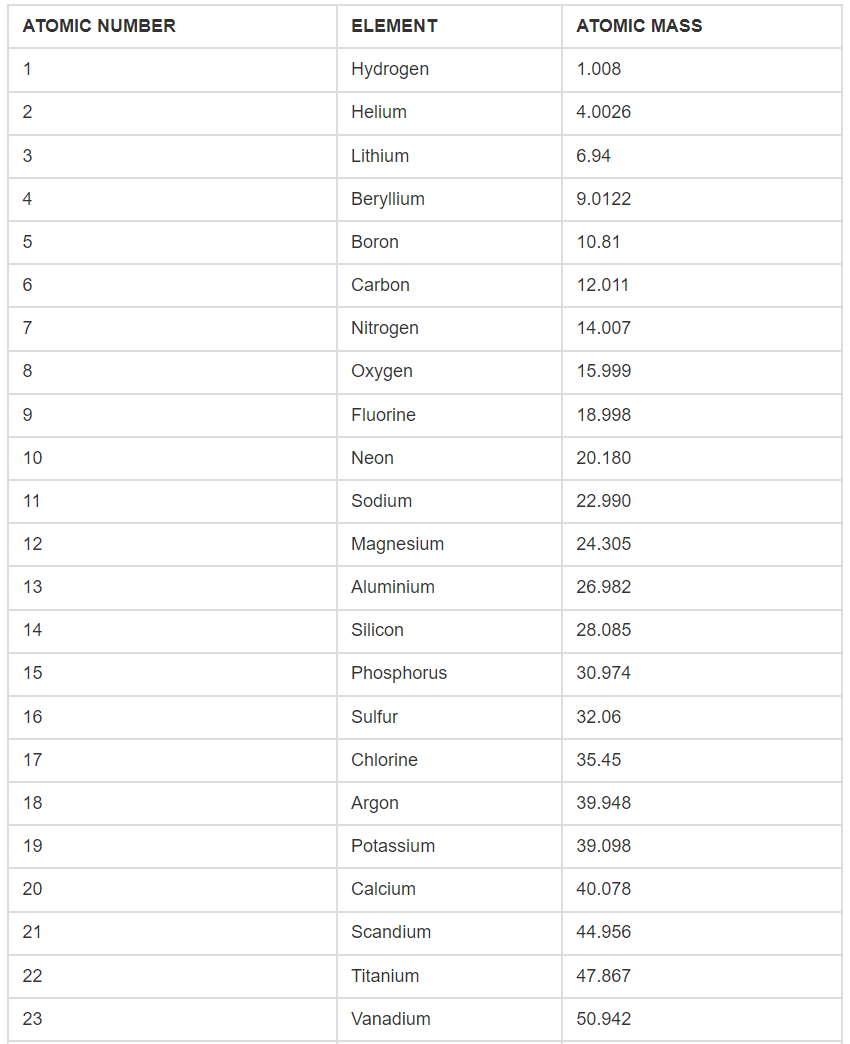
\includegraphics[scale=0.80]{amu.png}
\end{center}
\end{figure}
 

\end{document}
